% preamble and style file for M&R lecture slides
\documentclass[11.5pt,sans,english]{beamer}

\usetheme{EastLansing}
\usecolortheme{lily}

\usepackage[most]{tcolorbox}

\usepackage{verbatim}
%\usepackage{ulem}
%\usepackage{fontawesome}
%\usepackage{tikz}
%\usepackage{pifont}
%\usepackage{tabularx}
\usepackage{array,booktabs,xcolor,colortbl,multirow,rotating,amssymb}
%\usepackage{amsmath}
% \usepackage{vwcol}
% \usepackage[T1]{fontenc}

  
\newcommand\vect[1]{\underline{\mathbf{#1}}}
\newcommand\unitvect[1]{\hat{\boldsymbol{#1}}}
%\newcommand\hatdot[1] { \hat{ \dot{ \boldsymbol{#1} } } }

\newtcbox
{\keyc}{on line,arc=2pt, colback=yellow!30!white, colframe=yellow!30!black, before upper={\rule[-3pt]{0pt}{10pt} },boxrule=1pt,boxsep=0pt,left=6pt,right=6pt,top=2pt,bottom=2pt,}

\newtcbox
{\keyb}{on line,arc=1pt, colback=blue!30!white, colframe=blue!30!black, before upper={\rule[-3pt]{0pt}{10pt} },boxrule=1pt,boxsep=0pt,left=6pt,right=6pt,top=2pt,bottom=2pt,}

\newtcbox
{\keyl}{on line,arc=1pt, colback=pink!30!white, colframe=blue!30!black, before upper={\rule[-3pt]{0pt}{10pt} },boxrule=1pt,boxsep=0pt,left=6pt,right=6pt,top=2pt,bottom=2pt,}

\newtcbox
{\keyw}{on line,arc=1pt, colback=red!30!white, colframe=blue!30!black, before upper={\rule[-3pt]{0pt}{10pt} },boxrule=1pt,boxsep=0pt,left=6pt,right=6pt,top=2pt,bottom=2pt,}

\newtcbox
{\keya}{on line,arc=1pt, colback=purple!30!white, colframe=blue!30!black, before upper={\rule[-3pt]{0pt}{10pt} },boxrule=1pt,boxsep=0pt,left=6pt,right=6pt,top=2pt,bottom=2pt,}

\newtcbox[auto counter,number within=section]
{keyf}
{
enhanced,
on line,
  boxsep=0pt,
  left=6pt,right=6pt,top=2pt,bottom=2pt,
  arc=5pt,
  boxrule=1pt,
  rightrule=38pt,
colback=green!10!white, 
colframe=green!50!black, 
title=\thetcbcounter,
detach title,
overlay unbroken and first ={
    \node[%rotate=90,
          %minimum width=1cm,
          anchor=south,
          font=\sffamily\bfseries\tiny,
          %yshift=-10pt,
          yshift=-5pt,
          xshift=-20pt,
          white]
    at (frame.east) {\thetcbcounter};
  }
}


\usepackage{xcolor}

%\usepackage{hyperref}
%\hypersetup{
%  pdfauthor={Lily Asquith},
%  urlcolor=blue,
%  colorlinks=true,
%  linkcolor=blue,
%  bookmarks=true
%}

%---------------------------------------------%
%              LILY'S COLOURS           %
%---------------------------------------------%
\definecolor{Wash}{RGB}{204,204,204}
%\definecolor{Pinky}{RGB}{254,200,254}%violet
\definecolor{Pinky}{RGB}{219,	240,	253}%violet
\definecolor{Bluey}{RGB}{0,190,255}%deep sky blue
\definecolor{DarkGrey}{RGB}{28,66,137}%dar grey
\definecolor{SussexWhite}{RGB}{253,255,254}%dar grey
\definecolor{LightGray}{RGB}{184,184,255}
\definecolor{YesGreen}{RGB}{0,128,0}
\definecolor{NoRed}{RGB}{250,0,0}



\definecolor{myred}{RGB}{255,153,153}
\definecolor{myorange}{RGB}{255,204,153}
\definecolor{myyellow}{RGB}{255,255,153}
\definecolor{mygreen}{RGB}{153,255,153}
\definecolor{mycyan}{RGB}{153,255,255}
\definecolor{myblue}{RGB}{153,204,255}
\definecolor{myviolet}{RGB}{153,153,255}
\definecolor{mypurple}{RGB}{204,153,255}
\definecolor{mypink}{RGB}{255,204,255}
\definecolor{mycoral}{RGB}{255,153,204}

%-----------------------------------------------------%
%              LILY'S COLUMN TYPES          %
%-----------------------------------------------------%
\newcolumntype{a}{>{\raggedright\arraybackslash}l}	
\newcolumntype{q}{>{\raggedright\arraybackslash}m{8cm}} 

%--------------------------------------------%
%              LILY'S SYMBOLS          %
%--------------------------------------------%
\newcommand{\dfinger}{\large{\textcolor{black}{\ding{43}}}\scriptsize}
\newcommand{\dstar}{\large{\textcolor{black}{\ding{76}}}\scriptsize}
\newcommand{\dwrite}{\large{\textcolor{black}{\ding{45}}}\scriptsize}
\newcommand{\ddiamond}{\small{\textcolor{DarkGrey}{\ding{117}}}\scriptsize}
\newcommand{\ddiamondwhite}{\small{\textcolor{SussexWhite}{\ding{117}}}\scriptsize}
\newcommand{\experiment}{\small{\textcolor{magenta}{\faCogs }}\scriptsize}
\newcommand{\watchit}{\textcolor{blue}{ \faYoutube}}


\makeatletter
\newcommand\notsotiny{\@setfontsize\notsotiny{6.5}{7.5}}
\makeatother


% 
\title[ Intro to Quantum Physics]{Intro to Quantum Physics F3241}
%\subtitle{\textbf{Part 4: The Photoelectric Effect}}
\author[Dr Lily Asquith (Lily)]{ Dr Lily Asquith (Lily)}
\date[Week 7]{ Week 7}
\logo{

\includegraphics[width=1.5cm]{../../utils/uslogo.jpg}
}


\begin{document}


\begin{frame}
\titlepage
\end{frame} 


\section{I2Q Part 7: Rutherford}
 
 \begin{frame}{Recap Atomic Spectra}
\small
Different atoms, when excited, emit photons with different specific wavelengths.\\[1ex]

We have a formula for predicting the wavenumber (or wavelength) of photons absorbed/emitted by different atoms.\\[1ex]

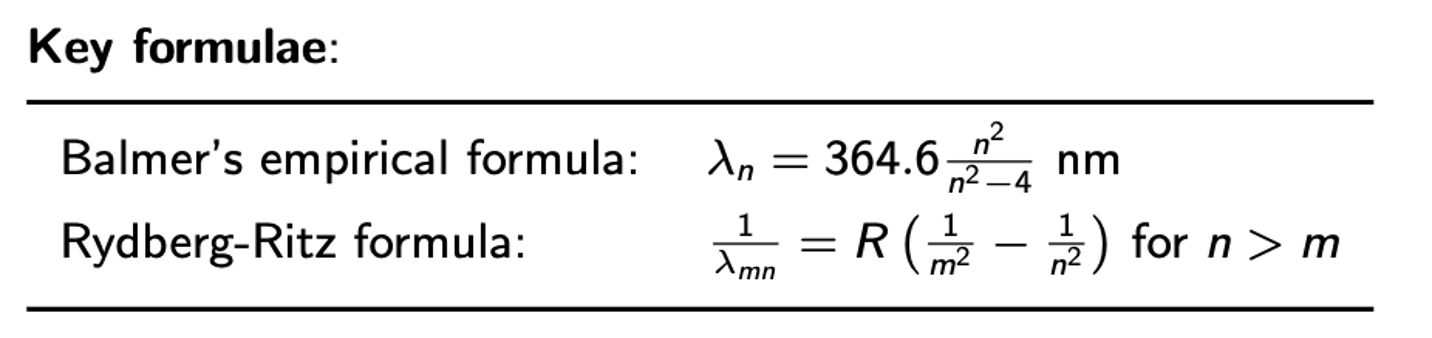
\includegraphics[scale=0.4]{recap-spectra}

\end{frame}

 \begin{frame}{Rydberg's formula for Hydrogen}
 \large

$\frac{1}{\lambda} = R[\frac{1}{m^2} - \frac{1}{n^2} ]$ for $n>m$\\[3ex]

\small
Rydberg's constant $R_{\infty} = 1.0974 \times 10^7$m$^{-1}$\\[3ex]

For Hydrogen, $R_{H} = 1.0968 \times 10^7$m$^{-1}$\\[3ex]

Hydrogen is different than all other atoms:\\[10ex]




\end{frame}

 \begin{frame}{Rydberg's formula in general}
\small
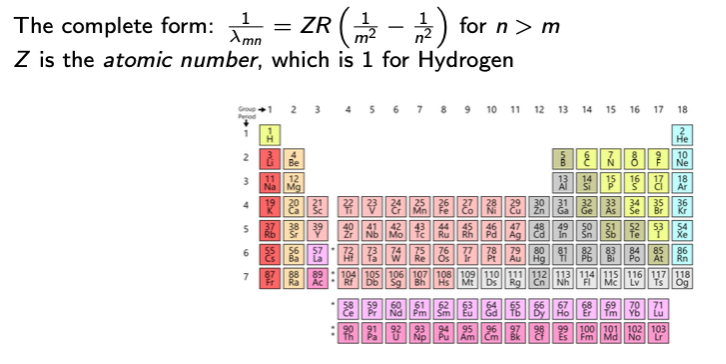
\includegraphics[scale=0.4]{spec9}

\end{frame}



 \begin{frame}{Collisions / scattering}
\small
Elastic Scattering:\\[10ex]

Inelastic Scattering:\\[10ex]


%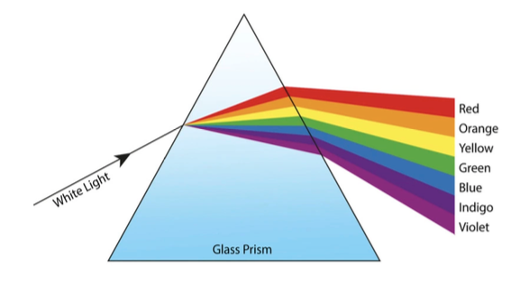
\includegraphics[scale=0.4]{spec1}

\end{frame}

 \begin{frame}{Why do atoms `prefer' to be in their ground state?}
\small
An excited atom will always return to its ground state via emission of a photon with a specific wavelength. Why?\\[25ex]


%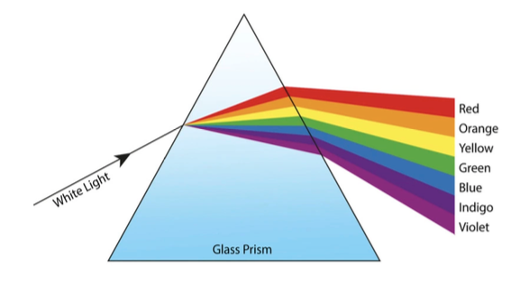
\includegraphics[scale=0.4]{spec1}

\end{frame}



 \begin{frame}{Rutherford Scattering}
\small


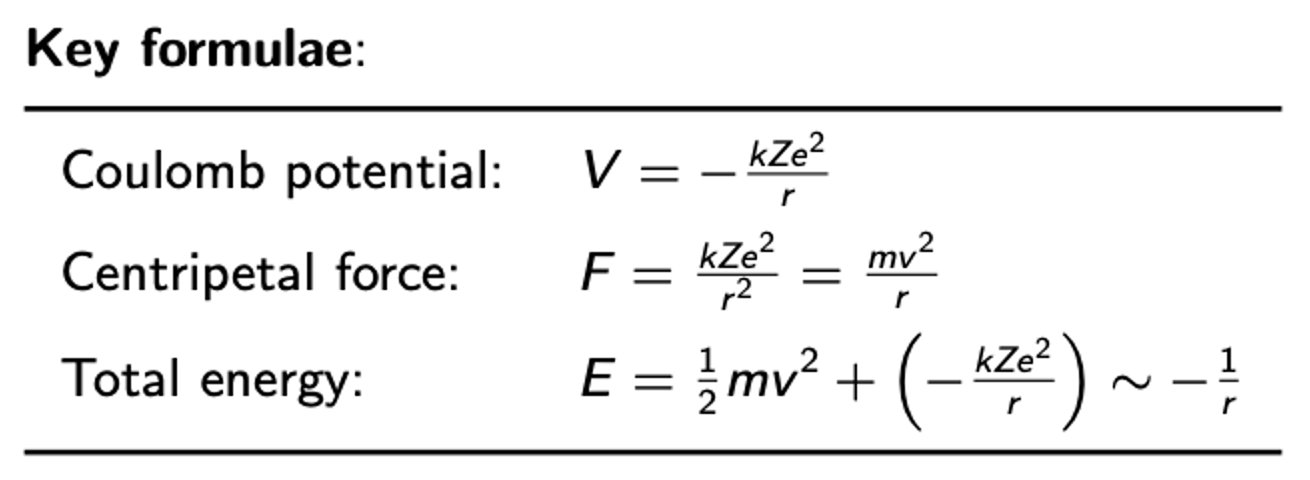
\includegraphics[scale=0.4]{ruth-form}

\end{frame}


 \begin{frame}{A whirlwind intro to electrodynamics}
\small
Coulomb's Law: $F = k \frac{q_1 q_2}{r^2}$\\[4ex]
1. Opposites attract.\\[2ex]
2. The electric force follows an inverse square law.\\[2ex]
3. The electric force is different depending on the medium in which the charges are placed.\\[2ex]
%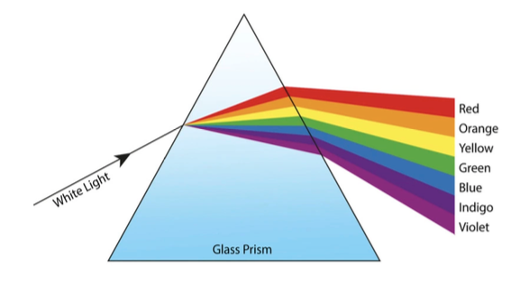
\includegraphics[scale=0.4]{spec1}
Coulomb's constant $k = \frac{1}{4\pi \epsilon_0} = 1.44 e^{-2}$ MeV fm\\[1ex]

\end{frame}


 \begin{frame}{A whirlwind intro to electrodynamics}
\small
Coulomb's Law: $F = k \frac{q_1 q_2}{r^2}$\\[4ex]
What is the potential energy associated with this force?\\[25ex]

%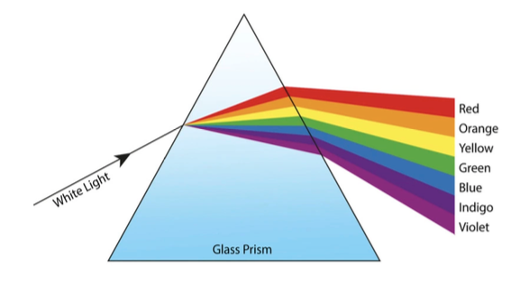
\includegraphics[scale=0.4]{spec1}

\end{frame}


 \begin{frame}{Thomson's Atom}
\small


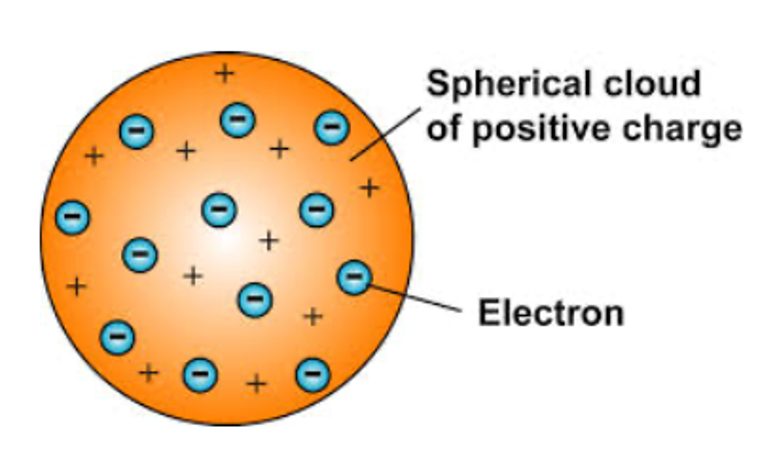
\includegraphics[scale=0.4]{thomson}

Rutherford: let's test this model by smashing charged particles into an atom!
\end{frame}


 \begin{frame}{Rutherford's Experiment}
\small


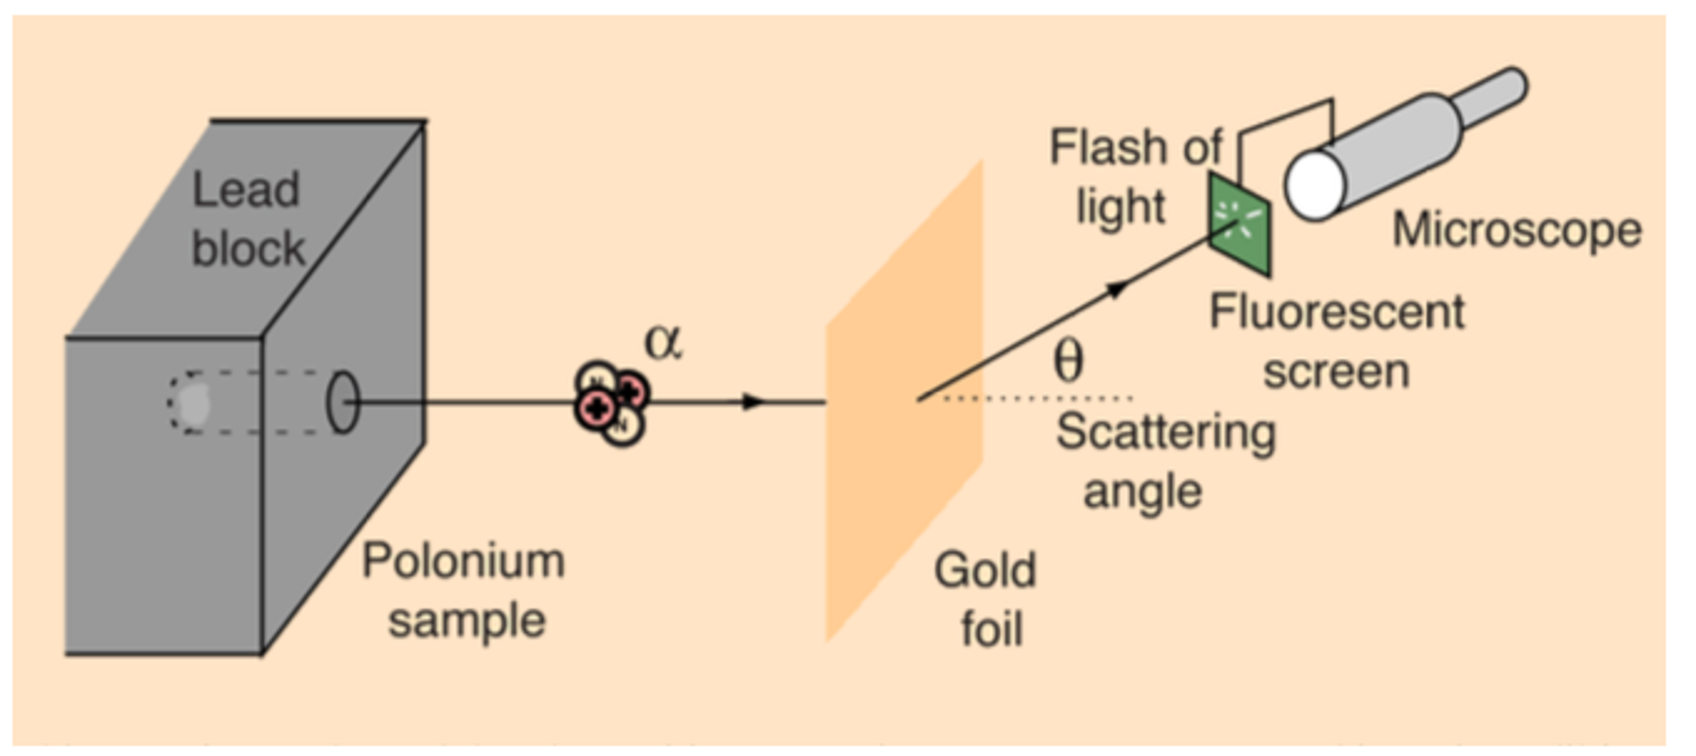
\includegraphics[scale=0.4]{ruthexp}

Rutherford observed some particles being back-scattered.
\end{frame}


 \begin{frame}{Conservation of momentum and KE (2-body)}
\small
Momentum is always conserved:\\[10ex]




Kinetic energy is only conserved in elastic collisions:\\[10ex]

%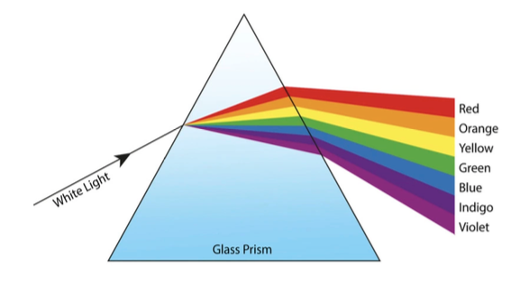
\includegraphics[scale=0.4]{spec1}

\end{frame}


 \begin{frame}{Conservation of total Energy}
\small
$(KE+PE)_i$ = $(KE+PE)_f$\\[4ex]

Initially:\\[10ex]


Finally:\\[10ex]



%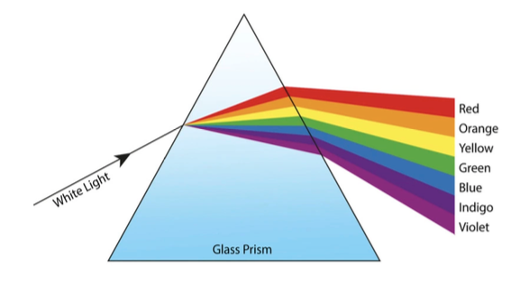
\includegraphics[scale=0.4]{spec1}

\end{frame}

 \begin{frame}{Rutherford's Formula}
\small


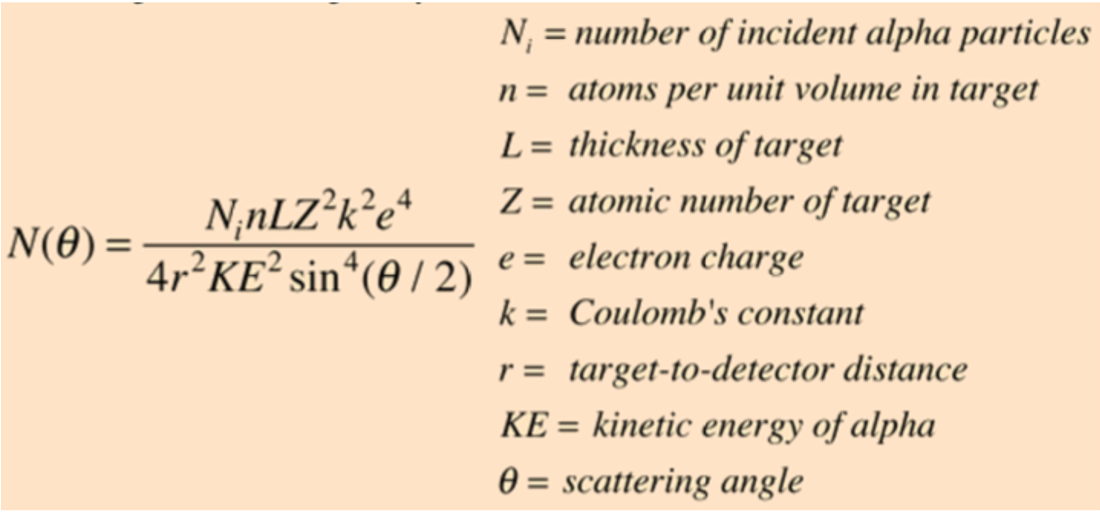
\includegraphics[scale=0.4]{ruthform}
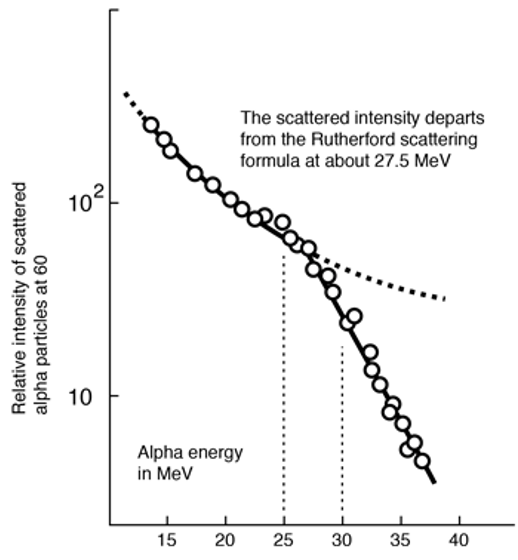
\includegraphics[scale=0.4]{ruthplot}

\end{frame}


 \begin{frame}{Higher Energy reveals Deeper Structure}
\small
10 MeV: An atom contains a nucleus!\\[3ex]

1 GeV: A nucleus contains nucleons! \\[3ex]

10 GeV: A nucleon contains partons! \\[3ex]

10 TeV: Now!\\[3ex]
%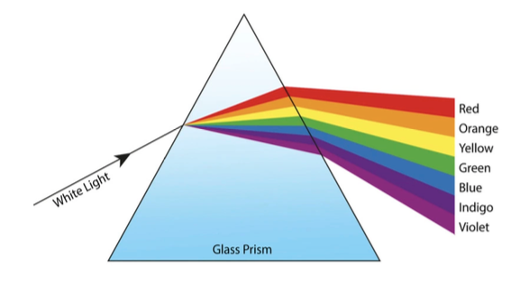
\includegraphics[scale=0.4]{spec1}

\end{frame}


 \begin{frame}{A Conundrum}
\small



%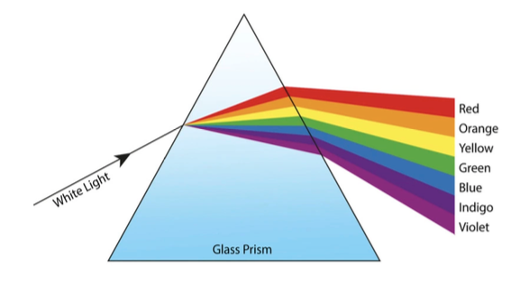
\includegraphics[scale=0.4]{spec1}

\end{frame}


\end{document}